\section{Authentication}
\subsection{Tổng quan}
Hệ thống  được xây dựng với các tính năng bảo mật cao, hỗ trợ đa dạng phương thức xác thực bao gồm:
\begin{itemize}
    \item Xác thực email thông qua verification code
    \item Quản lý phiên đăng nhập với JWT (Access token \& Refresh token)
    \item Chức năng quên và đặt lại mật khẩu
\end{itemize}
\subsection{Chi tiết triển khai}
\subsubsection{Quản lí token:}
Hệ thống sử dụng cơ chế JWT với 2 loại token:
\begin{itemize}
    \item \textbf{Access token:}
    \begin{itemize}
        \item Thời gian sống ngắn (mặc định 15 phút)
        \item Sử dụng SECRET\_KEY riêng để mã hóa
        \item Chứa thông tin user ID trong claim "sub"
        \item Có thể tùy chỉnh thời gian hết hạn
    \end{itemize}
    \item \textbf{Refresh Token:}
    \begin{itemize}
        \item Thời gian sống dài (cấu hình theo số ngày): 7 ngày
        \item Sử dụng REFRESH\_SECRET\_KEY riêng biệt
        \item Dùng để cấp mới access token khi hết hạn
        \item Tích hợp xử lý lỗi khi token hết hạn hoặc không hợp lệ
    \end{itemize}
\end{itemize}
\subsubsection{Các API endpoint}
\textbf{Xác thực email và đăng ký:}
\begin{itemize}
    \item \textbf{/verify-email:} Xác thực email thông qua mã code
    \begin{figure}[H]
        \centering
        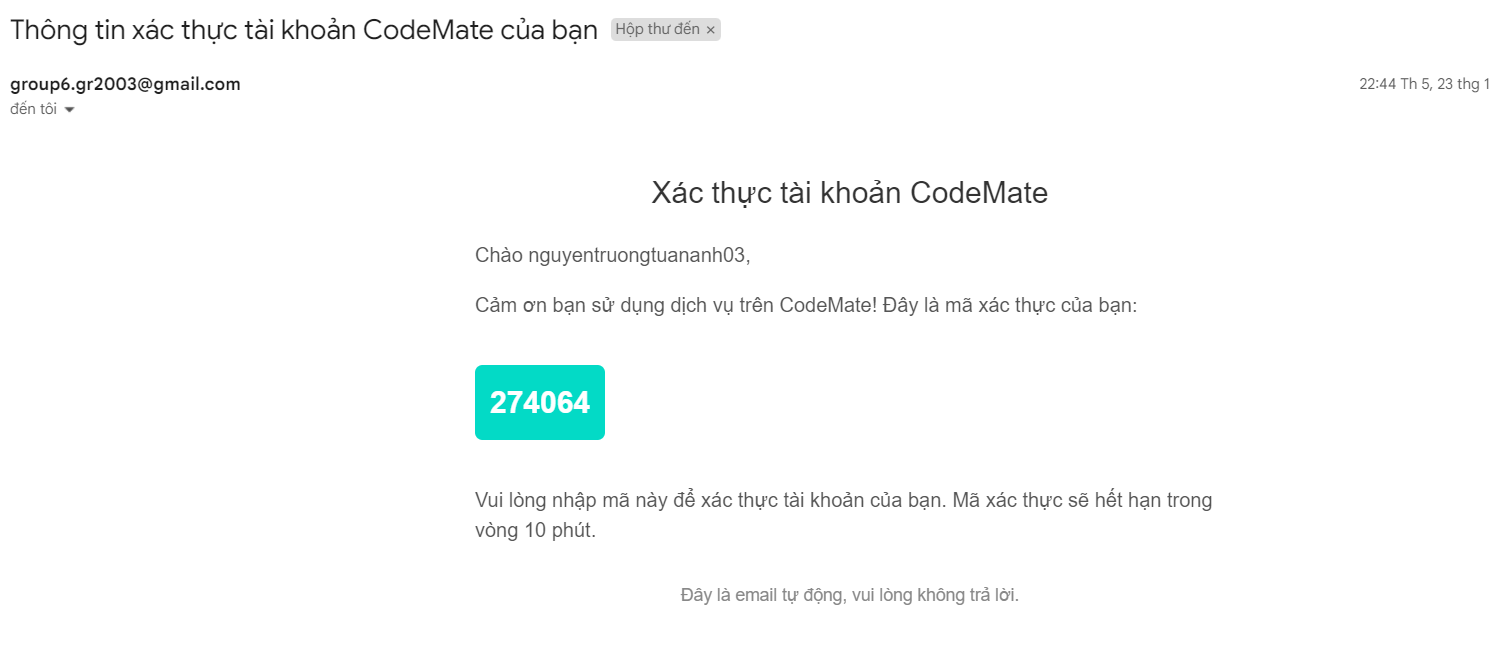
\includegraphics[width=0.8\linewidth]{images/verify_email.png}
        \caption{Xác thực email thông qua mã code}
        \label{fig:enter-label}
    \end{figure}
    \item \textbf{/resend-verification-code:} Gửi lại mã xác thực
\end{itemize}
\textbf{Quản lý Mật khẩu:}
\begin{itemize}
    \item \textbf{/forgot-password:} Khởi tạo quy trình quên mật khẩu
    \begin{figure}[H]
        \centering
        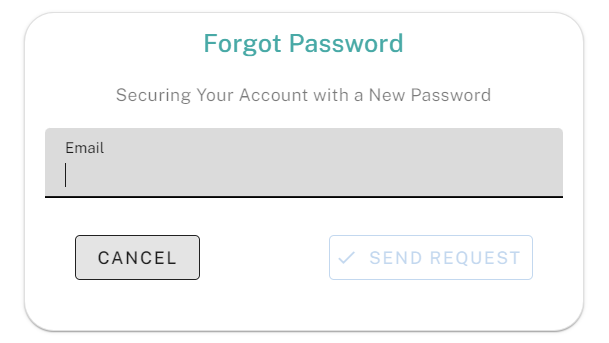
\includegraphics[width=0.6\linewidth]{images/forgot_password.png}
        \caption{Quên mật khẩu}
        \label{fig:enter-label}
    \end{figure}
    \item \textbf{/reset-password:} Đặt lại mật khẩu mới
    \item Sử dụng hash\_password để mã hóa mật khẩu an toàn
\end{itemize}

\section{Login}
\subsection{Tổng quan:}
Hệ thống có thể đăng nhập thông qua 2 phương thức:
\begin{itemize}
    \item Đăng nhập bằng email trường cấp (cho sinh viên và giảng viên)
    \item Đăng nhập với Google
\end{itemize}
\subsection{Chi tiết triển khai:}
\textbf{Trang giới thiệu:}
\begin{figure}[H]
        \centering
        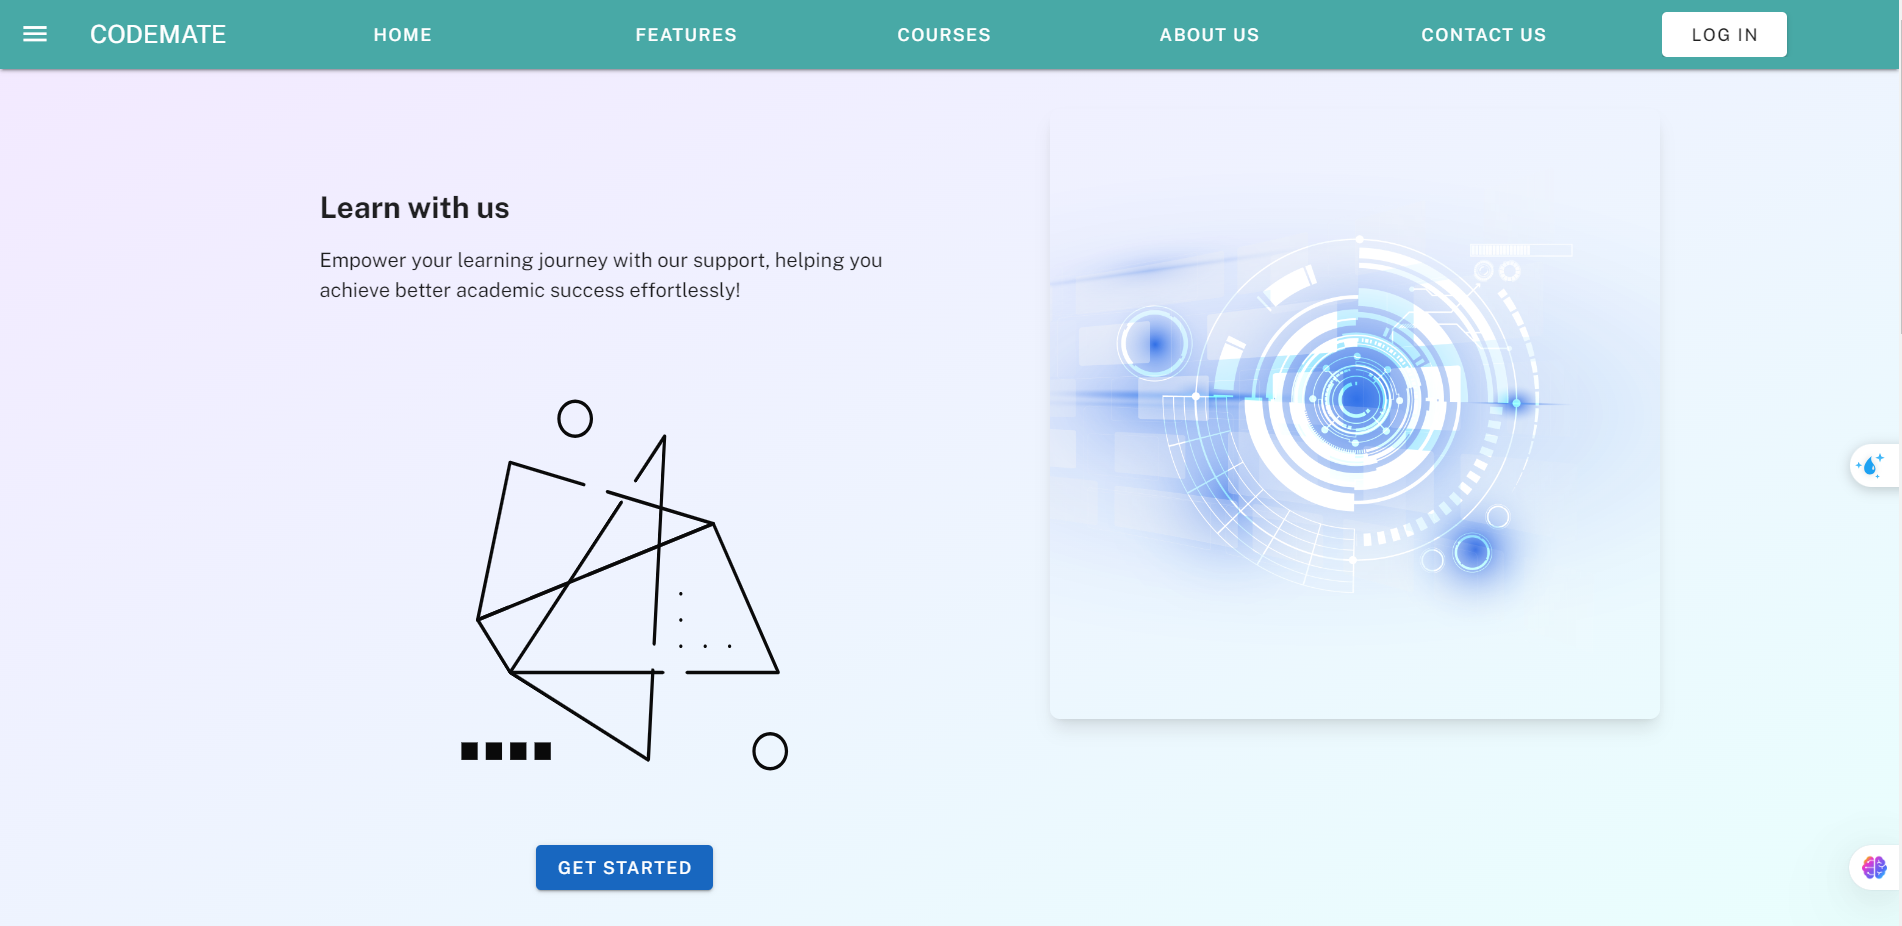
\includegraphics[width=0.8\linewidth]{images/introduction.png}
        \caption{Trang khởi đầu của hệ thống}
        \label{fig:enter-label}
    \end{figure}
\begin{figure}[H]
        \centering
        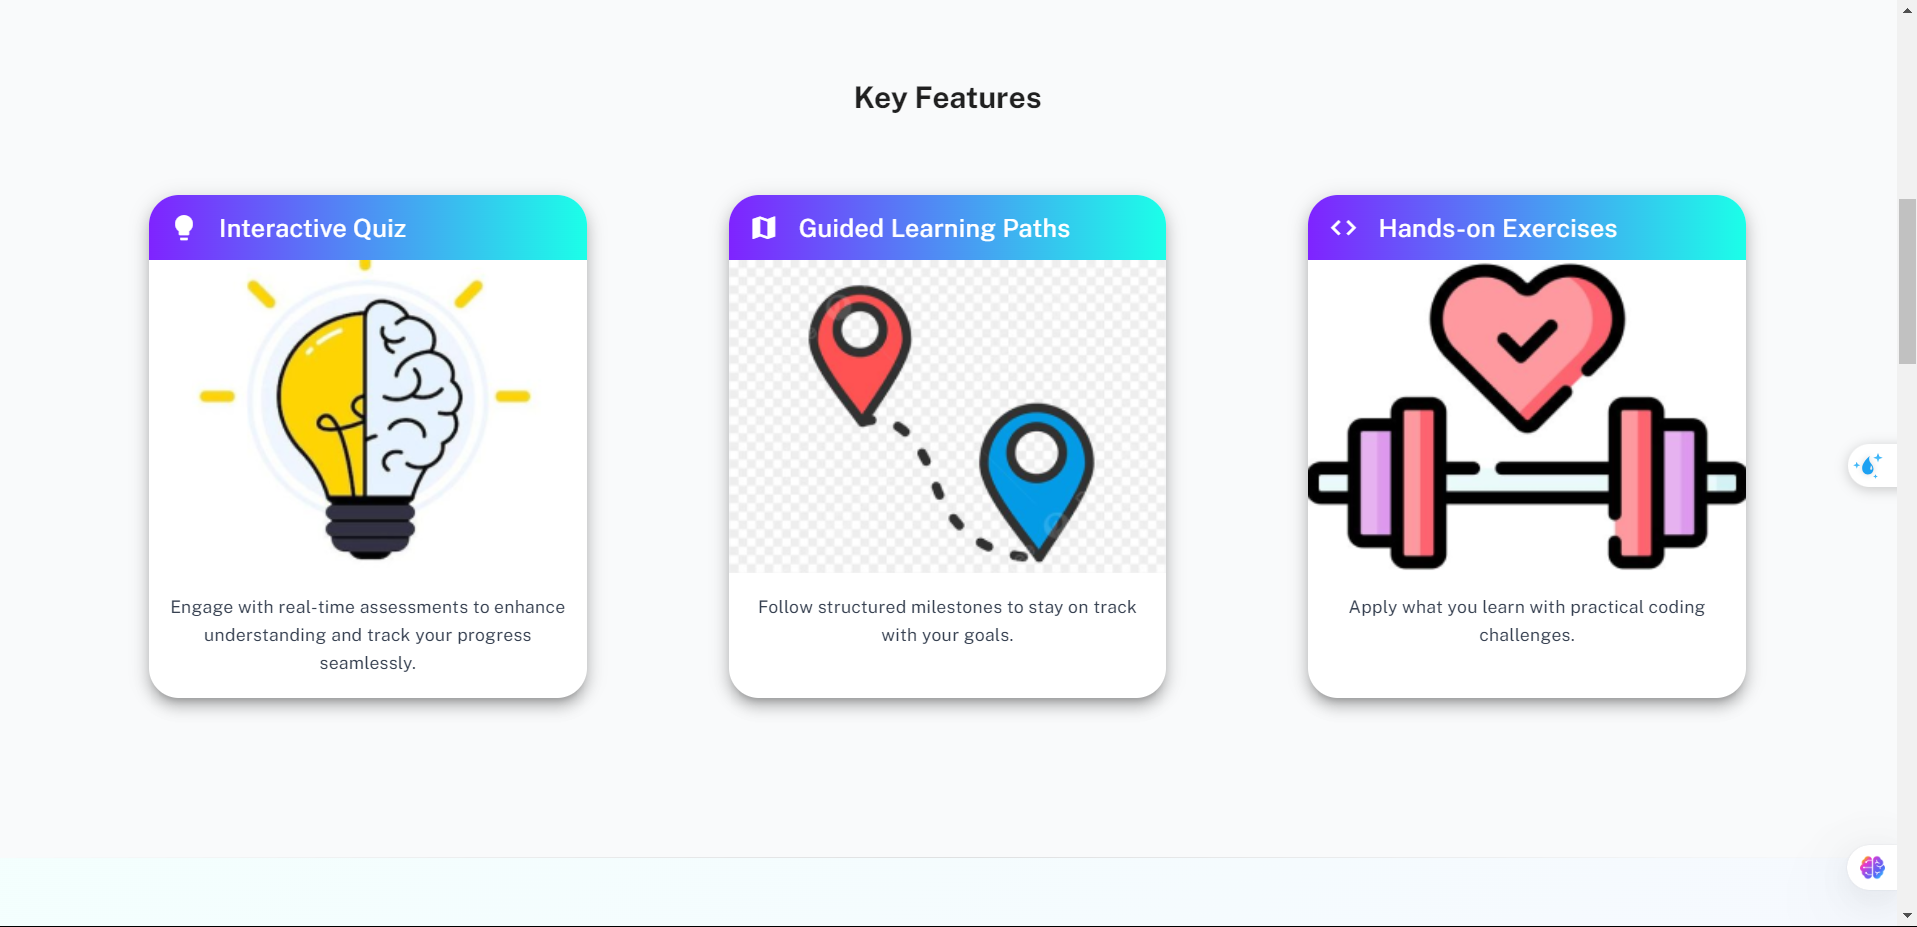
\includegraphics[width=0.8\linewidth]{images/introduction_feature.png}
        \caption{Giới thiệu các tính năng nổi bật}
        \label{fig:enter-label}
    \end{figure}
    \begin{figure}[H]
        \centering
        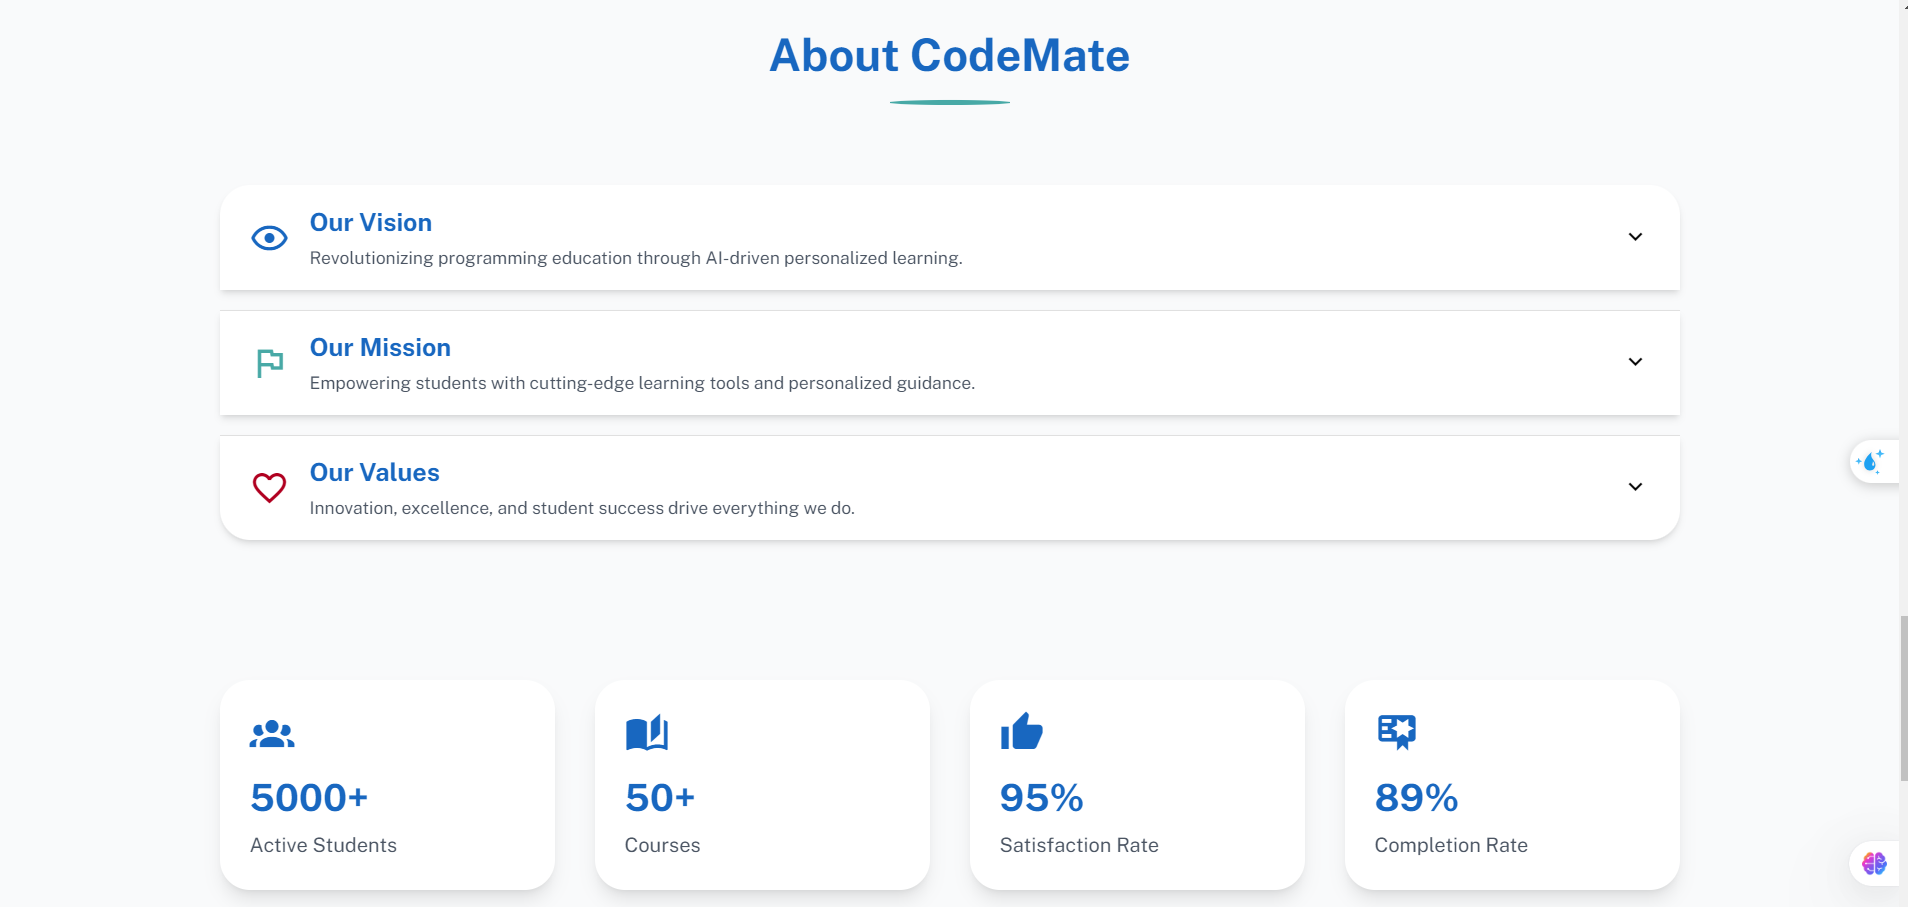
\includegraphics[width=0.8\linewidth]{images/introduction_about.png}
        \caption{Giới thiệu về hệ thống Codemate}
        \label{fig:enter-label}
    \end{figure}
    \begin{figure}[H]
        \centering
        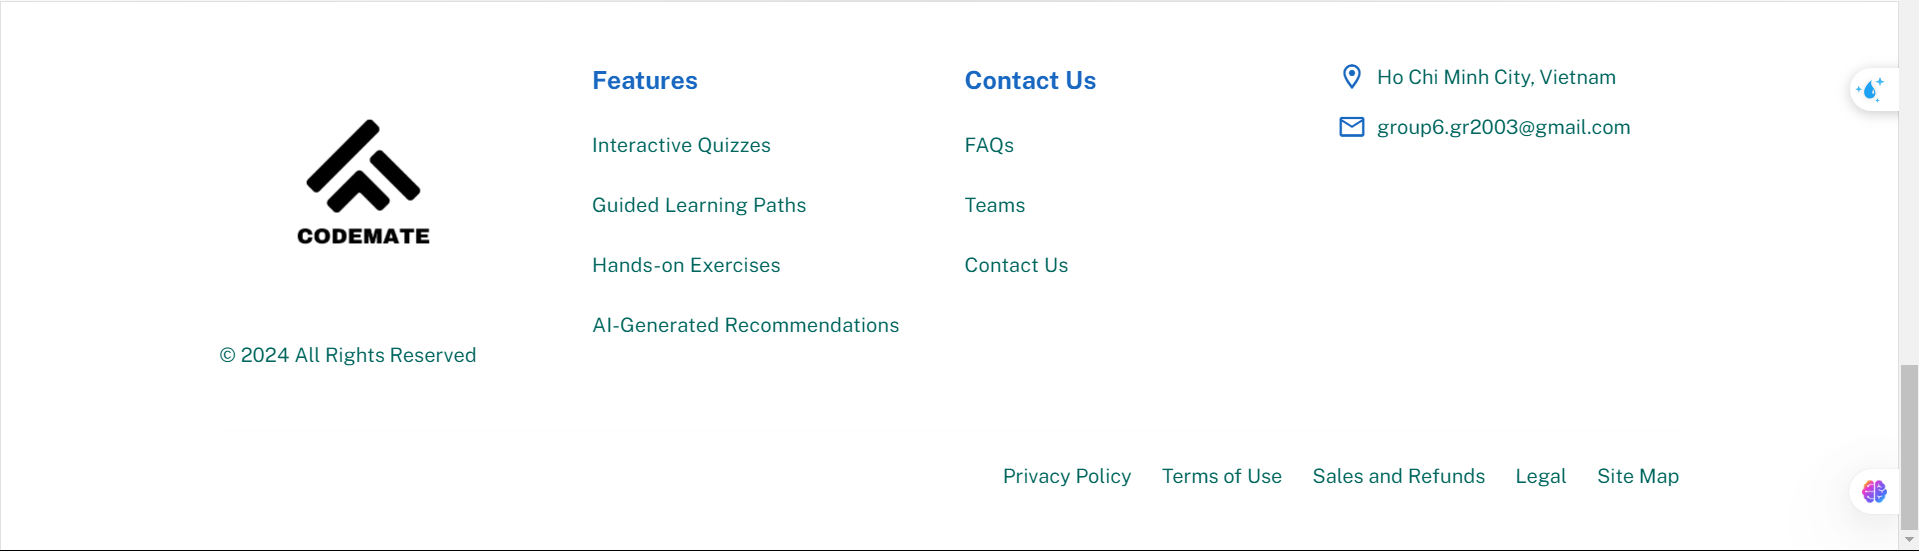
\includegraphics[width=0.8\linewidth]{images/introduction_contact.png}
        \caption{Thông tin liên hệ}
        \label{fig:enter-label}
    \end{figure}
\textbf{Đăng nhập bằng email trường:}
\begin{itemize}
    \item Kiểm tra thông tin đăng nhập: xác thực email và mật khẩu, định dạng email trường.
    \begin{figure}[H]
        \centering
        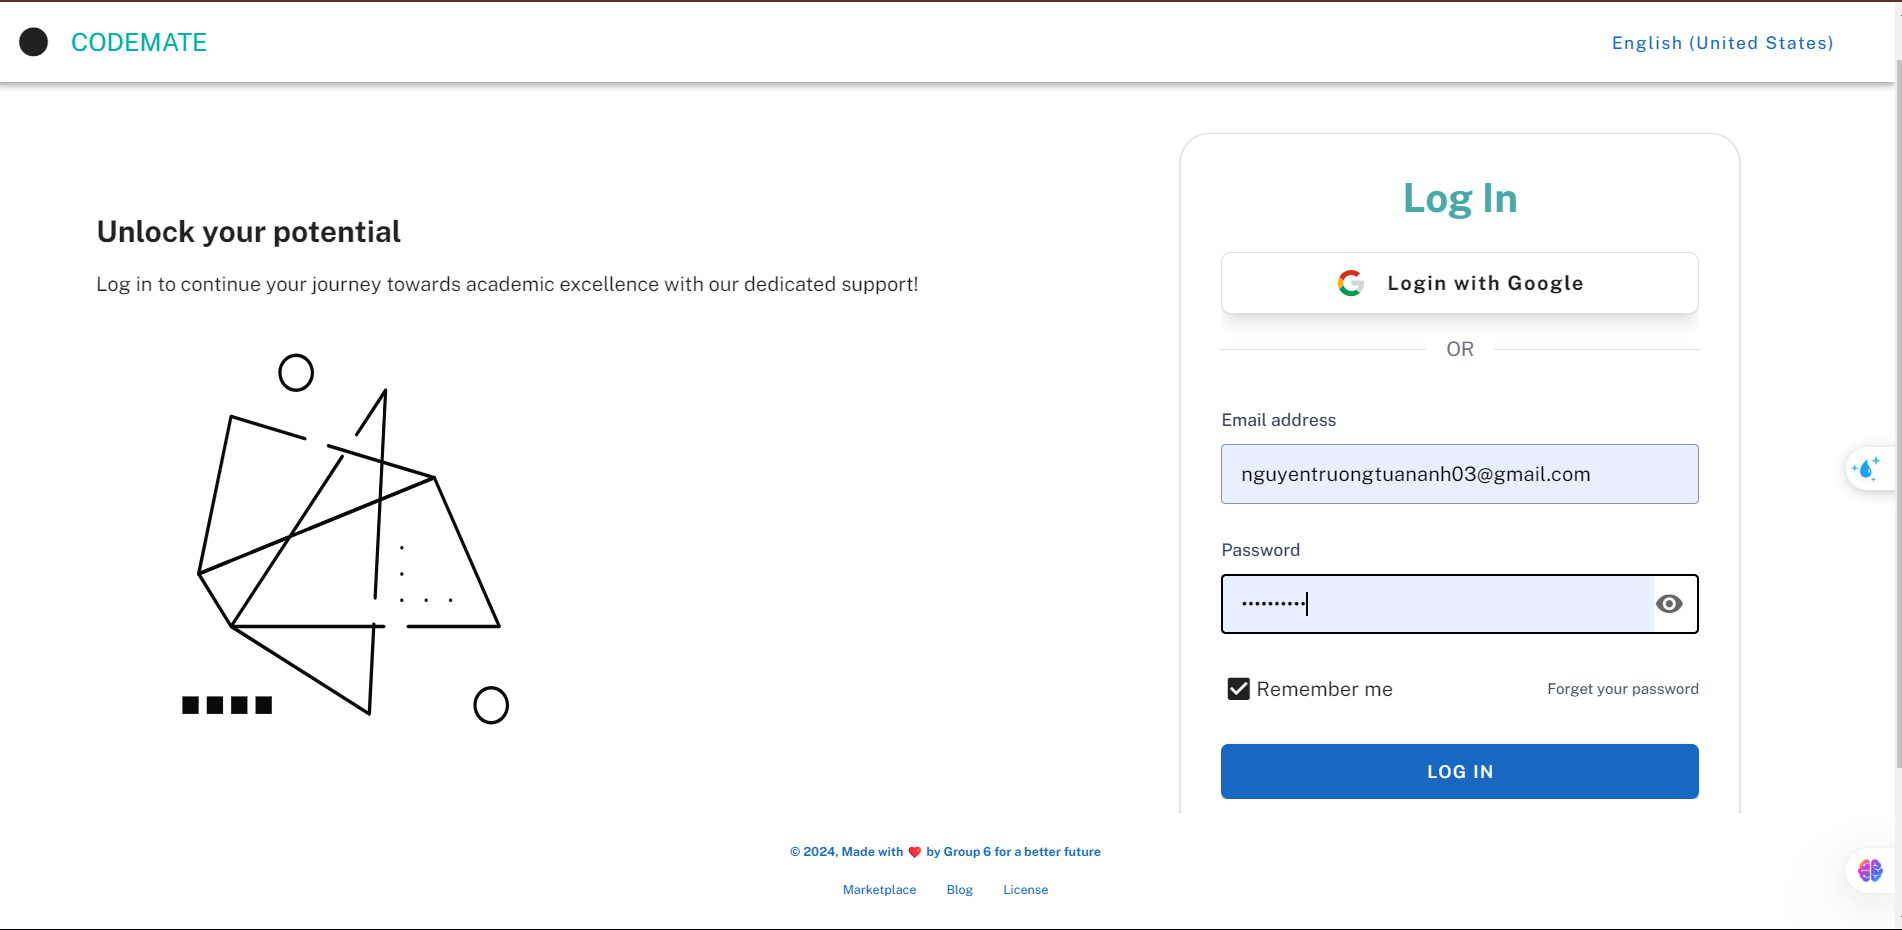
\includegraphics[width=0.8\linewidth]{images/login.png}
        \caption{Nhập tài khoản và mật khẩu}
        \label{fig:enter-label}
    \end{figure}
    \item Kiểm tra trạng thái xác thực email (is\_verified) nếu chưa tạo mã xác thực ngẫu nhiên gửi đến email người dùng.
    \begin{figure}[H]
        \centering
        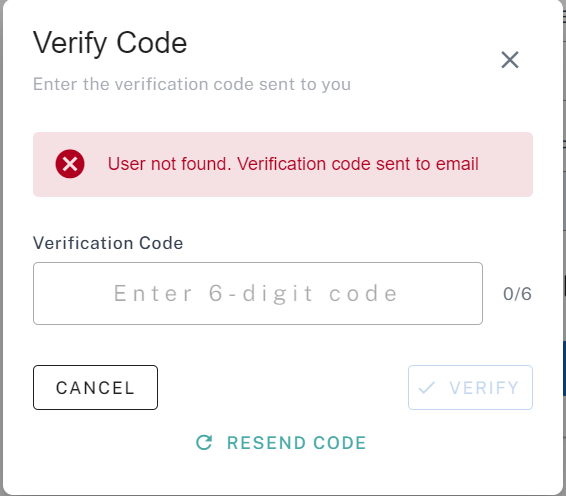
\includegraphics[width=0.6\linewidth]{images/send_code.png}
        \caption{Nhập mã code}
        \label{fig:enter-label}
    \end{figure}
    
    \item Phân quyền người dùng
\end{itemize}
